\documentclass{book}
\usepackage{amsmath}
\usepackage{bm}
\usepackage{colortbl}
\usepackage{graphicx}
\usepackage{caption}
\usepackage{fullpage}
\usepackage{afterpage}
\usepackage{multirow}
\usepackage{setspace}
\usepackage{booktabs}
\usepackage{gensymb}
\usepackage{parskip}
\usepackage{xr}
\usepackage{pdflscape}
\usepackage[inline]{enumitem}
\usepackage{wrapfig}
\usepackage{longtable}
\usepackage{subfig}
\usepackage[natbib=true, style=numeric-comp,subentry,backend=biber,sorting=none]{biblatex}
\addbibresource{citation/Thesis.bib}
\usepackage[hidelinks]{hyperref}
\usepackage{fancyhdr}
\usepackage{fixltx2e}
\usepackage{nomencl}




\pagestyle{fancy}
\fancyhead[LE,RO]{\itshape \nouppercase \rightmark}
\fancyhead[LO,RE]{\itshape \nouppercase Chapter \arabic{chapter}}
\setlength{\headheight}{40.0pt}
\setlength{\headsep}{0.2in}
\addtolength{\topmargin}{-4\baselineskip}
\renewcommand{\headrulewidth}{0.4pt}
\renewcommand{\footrulewidth}{0.4pt}
\newcommand{\beginsupplement}{%
	\setcounter{table}{0}
	\renewcommand{\thetable}{S\arabic{table}}%
	\setcounter{figure}{0}
	\renewcommand{\thefigure}{S\arabic{figure}}%
}

\title{Genetic and Environmental risk factors of Schizophrenia and Autism}
\date{\today}
\author{\href{mailto:choishingwan@gmail.com}{Choi Shing Wan}\\
	
\includegraphics[width=0.5\textwidth]{hkuLogo.jpg}}
\singlespacing
\renewcommand*\contentsname{Contents}
\onehalfspacing
%\doublespacing

\newcommand{\gene}[1]{\textit{#1}}
\newcommand{\organism}[1]{\textit{#1}}
\newcommand{\function}[1]{\textit{#1}}

%\includeonly{environmental_risk/er_chapter,supplementary_materials}

\makenomenclature
\makeindex
\begin{document}\thispagestyle{empty}
\pagestyle{empty}

%\maketitle
\begin{titlepage}
	\begin{center}
		\vspace*{1cm}
		
		\Huge
		\textbf{Genetic and Environmental risk factors of Schizophrenia and Autism}
		
		\vspace{0.5cm}
		\LARGE
		
		\vspace{1.5cm}
		
		\textbf{\href{mailto:choishingwan@gmail.com}{Choi Shing Wan}}
		
		\vfill
		
		A thesis submitted in partial fulfillment of the requirements for \\
		the Degree of Doctor of Philosophy
		
		\vspace{0.8cm}
		
		
\includegraphics[width=0.4\textwidth]{hkuLogo.jpg}
		
		\Large
		Department of Psychiatry\\
		University of Hong Kong\\
		Hong Kong\\
		\today
		
	\end{center}
\end{titlepage}


\frontmatter 

	\cleardoublepage
	\phantomsection
	\addcontentsline{toc}{chapter}{Declaration}
	\chapter*{Declaration}
	\cleardoublepage
	\phantomsection
	\addcontentsline{toc}{chapter}{Acknowledgments}
	\chapter*{Acknowledgements}
	\cleardoublepage
	\phantomsection
	\addcontentsline{toc}{chapter}{Abbreviations}
	\renewcommand{\nomname}{Abbreviations}
	%To generate the correct abbreviations, use alt+shift+F1 twice before using F1
	\printnomenclature
	
	\cleardoublepage
	\phantomsection
	\addcontentsline{toc}{chapter}{Contents}
	\begin{singlespace}
		\tableofcontents
	\end{singlespace}
\mainmatter
	\chapter*{Introduction}\pagestyle{fancy}
		\addcontentsline{toc}{chapter}{Introduction}
	\chapter[Literature Review I: Schizophrenia and Autism]{Literature Review I:\\ Schizophrenia and Autism}
		\section{Schizophrenia}
			Schizophrenia (SCZ)\nomenclature{SCZ}{Schizophrenia} is a %Description fo the disease%
			Affecting  roughly 1$\%$ of the human population.
			Detrimental to the quality of life.
			Limited treatment.
			No cure.
			\textbf{Detail description of the disease here}
		\section{Autism Spectrum Disorder}
			On the other hand, Autism Spectrum Disorder\nomenclature{ASD}{Autism Spectrum Disorder}
			Affecting XXX of the population.
			Associated with mental retardation.
			Most are unable to take care of themselves.
			No cure.
			\textbf{Detail description of the disease here}
		\section{The Environmental Risk Factors of SCZ and ASD}
			Despite the difference in their phenotype, epidemiological studies suggest that they share a lot of common environment factors.
			\subsection{Prenatal Infection}
			Arguably one of the most important environmental risk factor for SCZ and AD. 
			Affect $\frac{1}{3}$ of all SCZ patient.
			Epidemiological study of Brown.
			The Involvement of IL-6.
			No protein found in the fetus.
			Talk about the finding of Oskvig and Smith.
			Imbalance caused by trying to counter the infection
			\subsection{Parental Age}
			\subsection{Prenatal Stress}
			\subsection{Maternal Vitamin D Deficiency During Pregnancy}
		\section{The Genetic Etiology of SCZ and ASD}
			Talk about the PGC studies.
			Previous line of evidence?
			What they have found with the genetic studies?
			(SCZ)
			Involvement of the PSD95. (Shaun)
			Most enriched area is the MHC.
			Other associated SNPs are also highly enriched by immune genes.
			(ASD)
			Need to read more paper on this
		\section{Summary}
	
	\chapter[Literature Review II: Approaches to Reveal Genetic Causes]{Literature Review II:\\ Approaches to Reveal Genetic Causes}
		\section{Twin Studies - Delineating Genetic and Environmental Contribution}
			Should briefly talk about how Twin modeling was used for finding the GE contribution.
			Should also mention the ACE model.
			At the end, we can talk about the heritability estimates of SCZ and AD
		\section{Searching for Genetic Variants}
			\subsection{Role of Common Variants}
				\subsubsection{Genome Wide Association Study}
					Should talk about what is GWAS and how it is used.
					Should also talk about the current GWAS studies in SCZ and AD
			\subsection{Role of Rare Variants}
				\subsubsection{Exome Sequencing}
					Similar to the GWAS.
					Talk about the Pros and Cons.
					Need to briefly mention the Denovo paper and Shaun's paper.					
				\subsubsection{Whole Genome Sequencing}
					Very very brief description of WGS and the current status.
				
		\section{Searching for Gene-Environmental interaction}
			\subsection{Gene Expression}
				\subsubsection{Micro-array}
				\subsubsection{RNA Sequencing}
				
			\subsection{Epigenetics}
				\subsubsection{Methylation Chip}
				\subsubsection{Bisulfite Sequencing}
		\section{Summary}
	


	\chapter[Environmental Risk Factor]{Environmental Risk Factor:\\ Maternal immune activation}
\section{Study Design}
This should serves as the place where we place the mini introduction.
What have people not done? early MIA. 
What is the importance? Earlier the worst.
What are we going to do?
What is the aim and goal?
Brief description of what to be done.
\section{Materials and Method}
%\externaldocument{environmental_risk/er_rtPCR_primer.tex}

\subsection{Mouse model}
\subsubsection{Sample Collection}
Two pregnant female C57BL/6N mice were obtained from the University of Hong Kong Laboratory Animal Unit (HKU-LAU).
Both animals were housed at standard temperature (21$\pm$1\degree C ) and humidity (55$\pm$5$\%$ ) under normal light-dark conditions (12 hours light/12 hours dark with lights on between 7:00 and 19:00).
Food and water were available \textit{ad lib}.
All experimental protocols were approved by the Committee on the Use of Live Animals in Teaching and Research at \gls{hku} (CULATAR 3070-13) and also from the Department of Health, Hong Kong Special Administrative Region (12-731) and were carried out in accordance with the approved guidelines. 

The day on which the vaginal plug was found was designated as \gls{gd} 0.
On \gls{gd} 9, one pregnant mouse was randomly assigned as case and received a single dose of \gls{polyic} (5mg/kg) via the tail vein under mild physical restraint, whereas the control mouse received a single dose of 0.9$\%$ saline (5ml/kg) \citep{Li2009c}.
The pregnant dams were sacrificed by cervical dislocation, 6 hours after the injection and fetuses were extracted individually.
A cut was made posterior to the fourth ventricles under the dissecting microscope to separate the head of each fetus \citep{Kaufman1992}, which was then frozen immediately in liquid nitrogen until RNA extraction. 


\citet{Meyer2006b} demonstrated that \gls{polyic} administration will leads to a marked increase in maternal serum cytokine levels of IL-1$\beta$, IL-6, IL-10 and TNF-$\alpha$.
Starting from 3 hours after the injection, it was observed that the fetal brain IL-6 level significantly increases and a marked decrease of fetal IL-1$\beta$ level was also observed. 
6 hours after the injection, the level of IL-6 remains elevated with the IL-1$\beta$ become significantly elevated when compare to that of the control samples.
Interestingly, this change is only observed in the \gls{gd}9 samples but not the \gls{gd}17 samples, suggesting that to be a specific change relevant to \gls{gd}9.
Thus, we selected the 6 hour time point for the fetal brain extraction in the hope to observe the immediate effect of PolyI:C insult to the fetal brain expression pattern.

\subsubsection{DNA Extraction and Foetal Sexing}
As a pilot study, we would like to focus our analysis only on the male fetus.
However, due to the early gestation day, where the genital system of the mouse has yet developed, sexing becomes almost impossible using the genital method.
To identify the sex of the fetus, \gls{pcr} were performed on genes presented on the sex chromosomes (XY) based on the protocol suggested by \citet{Clapcote2005a} to determine the sex of the fetus. 
Genomic DNA was extracted from the bodies of the fetuses, which were kept separately, using the TIANamp Genomic DNA kit (Tiangen, Cat. no. DP304) following the manufacturer's instructions.
The fetuses were then sexed by \gls{pcr} using primers as described in \citet{Clapcote2005a}.
 7 out of 10 fetuses from the \gls{polyic} dam and 5 out of 8 fetuses from the Saline dam were male.


\subsection{RNA Sequencing}
\subsubsection{RNA Extraction, Library Construction and Sequencing}
Total RNA was extracted from each fetal brain using RNeasx10-Micro-Kit (Qiagen, Cat. No. 74004) following the manufacturer’s instructions. 
RNA quality was assayed using the Agilent 2100 Bioanalyzer and RNA was quantified using the Qubit 1.0 Fluorometer. 
Samples with an \gls{rin} $\ge$ 9.5 were selected for sequencing (5 cases, 5 controls). 
The RNA-Seq library was performed at the Centre for Genomic Sciences, HKU, using the TruSeq Stranded mRNA Sample Prep Kit. 
The \gls{ercc} spike-in control \citep{Jiang2011a} was included as an internal control. 
All samples were sequenced using Illumina Hiseq at two lanes (2 $\times$ 101 bp paired-end reads) at Macrogen.

\subsubsection{Differential Gene Expression Analysis and Functional Enrichment}
%Should I also compare the performance of different alignment tools and DE analysis tools?

The sequence reads were subject to \gls{qc} using FastQC \citep{Andrews} and mapped to the \textit{Mus musculus} reference genome (mm10, Ensembl GRCm38.74) and ERCC reference using the STAR aligner (version 2.3.1v) \citep{Dobin2013}.
The read count per gene for each sample was calculated with HTseq (version 0.5.4p5) \citep{Anders2015}.
Differential gene expression analysis was performed using the DESeq2 package (version 2.1.4.5) \citep{Anders2010}.
In order to reduce noise associated with low expression, genes with base mean count $<$ 10 were removed from all analyses.
Outliers were replaced using the \textit{replaceOutliersWithTrimmedMean} function in DESeq2 \citep{Anders2010}. 
Genes with p-value passing the Bonferroni corrected p-value $<$ 0.05 were defined as \glspl{deg}. 

\gls{go} based enrichment analysis of \glspl{deg} was performed using GOrilla \citep{Eden2009}, which takes a list of \glspl{deg} as input and tests whether a particular \gls{go} term is overrepresented in the input list when compared to the background gene list.
Up-regulated and down-regulated gene lists were input separately such that we may identify \gls{go} terms corresponding to the up- and down-regulated gene lists.
As GO terms tends to be redundant and overlaps with each other, it will aid the interpretation of GO results based by clustering and reducing the GO terms based on their similarity. 
Thus, \gls{go} enrichment results were summarized by REViGO \citep{Supek2011} and significant representative \gls{go} terms were obtained.
Gene set enrichment analysis was conducted using the \textit{userListEnrichment} \citep{Miller2011} function in R to identify known brain-related gene sets enriched by the DEGs.
A description of these brain-related gene sets can be found in \url{http://www.inside-r.org/packages/cran/WGCNA/docs/userListEnrichment}.
Only gene sets with a Bonferroni corrected p-value $<$ 0.05 were considered as significant. 

\subsection{Combining with External Microarray Controls}
%Need to explain why we perform this analysis
We repeated all analyses mentioned above using control microarrays \gls{gd}9 C57BL/6 mouse fetal brain expression data (N=5) from \gls{geo} (GSE8091 \citep{Hartl2008}) obtained using GEOquery (version 2.30.0) \citep{Davis2007}.
In order to remove effects due to platform differences, our RNA-Seq data was first variance stabilized (\textit{varianceStabilizingTransformation} function in DESeq2\cite{Anders2010}) and then combined with the \textit{rma} normalized microarray data using the Combat algorithm \citep{Johnson2007} under the sva package (version 3.10.0) in R.
Scripts used in all analyses are available online at \url{https://github.com/choishingwan/RNA-Seq-Analysis}. 

\subsection{Burden of Genetic Risk Variants in Brain-Related Gene Sets}
To establish the Proof of Concept that the enriched brain-related gene sets discovered are relevant to schizophrenia and other neuropsychiatric diseases in humans, we tested for 
\begin{enumerate*}[label=\roman*)]
	\item whether there was an excess of reported \textbf{rare} \textit{de novo} genetic mutations in these gene sets in previous studies of autism and schizophrenia patients \citep{Fromer2014,ORoak2012,Sanders2012,Neale2012} using a hyper geometric test; and
	\item whether there was greater evidence of association of \textbf{common} genetic variants with schizophrenia \citep{Ripke2013} and autism \citep{Anney2010a} in these gene sets then in the genome as a whole using a set analysis algorithm \citep{Ideker2002}. 
\end{enumerate*}
Briefly, p-values of genes were first converted into a z-score $z_i$. 
To produce the z-score for each individual gene sets, we sum the z-score within each individual gene sets $z_{gene\ set} = \sum_i^kz_i$ where $k$ is the number of genes within the specific gene set. 
To obtain the background distribution, we construct 10,000 random gene sets of size $k$ using permutation. 
We can then calculate the mean $z_\mu$ and standard deviation $z_\sigma$ of z-score for gene sets of size $k$.
Therefore, we can calculate the significance of enrichment of the gene set as
$$
S_{gene\ set}=\frac{z_{gene\ set}-z_\mu}{z_\sigma}
$$
Which allow us to obtain the p-value using $S_{gene\ set}$. 
The script for this analysis can be also be found at \url{https://github.com/choishingwan/RNA-Seq-Analysis}. 


\subsection{Real time PCR (RT-PCR) validation}
We validated the RNA-Seq results using \gls{rtpcr} on the same samples plus six additional samples from two independent dams (Saline = 8, PolyI:C = 8).
Unfortunately, due to the small tissue size, there were only enough materials for 5 genes for \gls{rtpcr}. 
Therefore, 4 \glspl{deg} (\textit{Akt3}, \textit{Eomes}, \textit{Lama5} and \textit{Robo3}), together with the reference $\beta$-Actin(\textit{Actb}) were selected. 
Primers (designed by Invitrogen) are listed in Table \cref{suppleTab:rtPCR}. 
cDNA was synthesized using SuperScript III reverse transcriptase (Invitrogen). 
RT- PCR was performed by using 2$\mu$l of cDNA product in each reaction on the ABI prism 7900HT Sequence Detection System.
All reactions were run in triplicate and \gls{ct} values for the four genes were normalized with $\beta$-Actin (\textit{Actb}) as the reference. 
A Student’s T-test was performed to compare the normalized \gls{ct} values between the \gls{polyic} fetuses and the saline fetuses for each of the four genes \citep{Yuan2006}.

\section{Results}
\subsection{Quality Control and Alignment}
Figure \ref{fig:schematicMIA} summarizes the overall study design and results obtained.
On average, 39 million reads were generated for each sample. 
Over 90$\%$ of reads were uniquely mapped to the \textit{Mus musculus} reference genome (mm10, Ensembl GRCm38.74) and the ERCC spike-in control reference using STAR\cite{Dobin2013}. 
Read counts of the External RNA Controls Consortium (ERCC) spike-in control were highly correlated with their true concentration (Pearson’s R $\le$ 0.956)(Table \ref{tab:ercc_correlation}), indicating that the RNA Seq read counts were representative of the true mRNA concentration.
\begin{figure}[htbp]
	\centering
	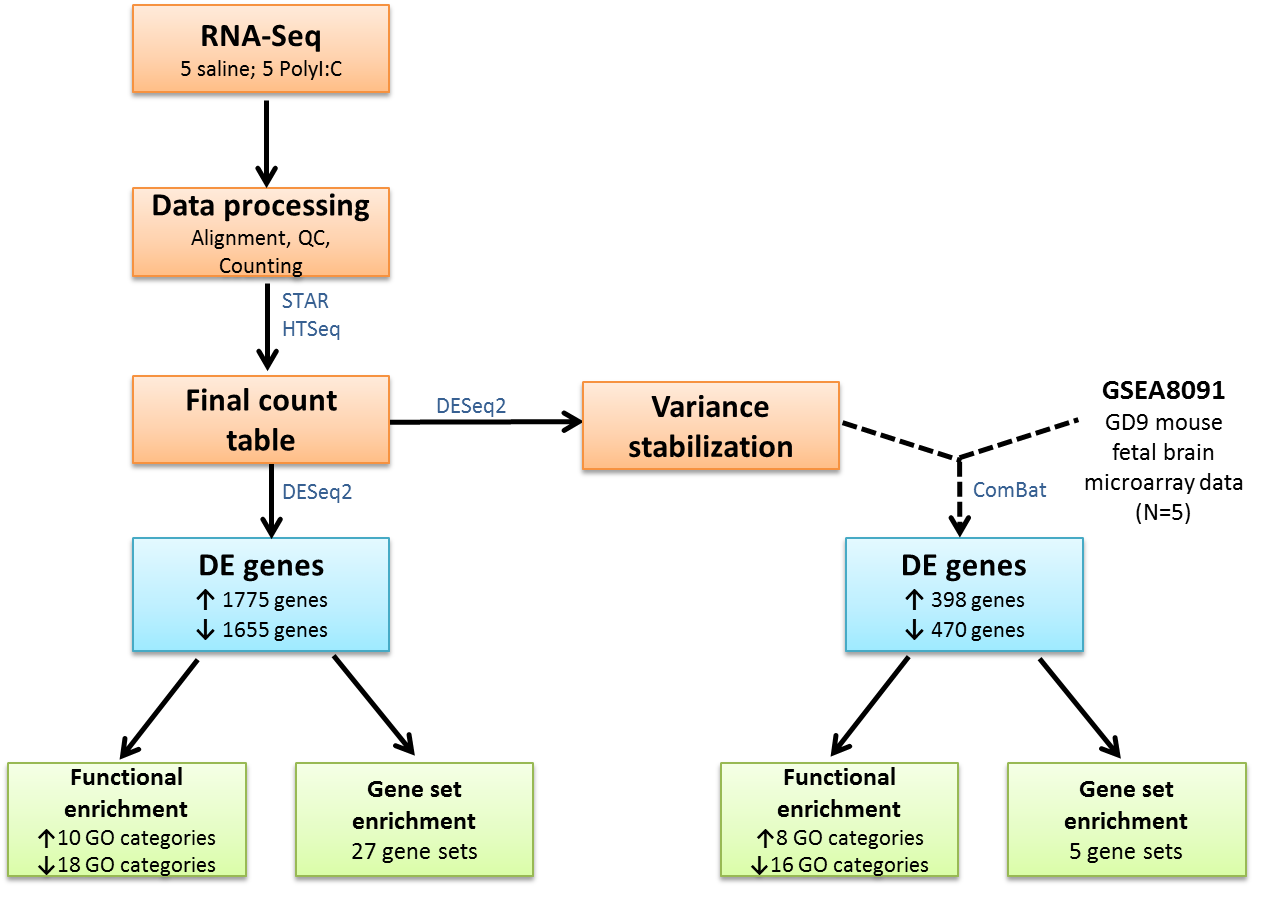
\includegraphics[width=0.9\textwidth]{environmental_risk/image/er_flowchart.png}
	\caption[Schematic of the experimental flow]{Schematic of the experimental flow. 
		Fetal mouse brains were extracted and used for RNA Sequencing. 
		DESeq2 were used to generate the differential expressed gene (DEG) list and also stabilize the variance of the gene expression counts. 
		Functional enrichment analysis were then performed on the DEG list using GOrilla, REViGO and the userListEnrichment function. 
		Stabilzed gene counts were then merged with the external microarray control using ComBat where the differential expression analysis and functional enrichment were again performed}\label{fig:schematicMIA}
\end{figure}
\begin{table}[h]
	\centering
	\caption[Correlation between concentration and counts]{Correlation between the true concentration and the normalized RNA Seq read counts.
		The high correlation indicates that the RNA Seq read counts are representative of the true concentration.}
	\label{tab:ercc_correlation}
	\begin{tabular}{rr}
		\toprule
		& \textbf{True Concentration} \\
		\midrule
		\textbf{Case 1} & 0.964 \\
		\textbf{Case 2} & 0.969 \\
		\textbf{Case 3} & 0.968 \\
		\textbf{Case 4} & 0.960 \\
		\textbf{Case 5} & 0.963 \\
		\textbf{Control 1} & 0.967 \\
		\textbf{Control 2} & 0.964 \\
		\textbf{Control 3} & 0.960 \\
		\textbf{Control 4} & 0.959 \\
		\textbf{Control 5} & 0.966 \\
		\bottomrule
	\end{tabular}%
\end{table}
\\
\\



\subsection{Differential gene expression analysis}
A total of 16,015 genes passed QC, of which 3,430 genes were differentially expressed (1,775 up-regulated and 1,655 down-regulated) with a Bonferroni-corrected p-value $<$ 0.05. 
A volcano plot of PolyI:C versus Saline for all genes is presented in Figure \ref{subfig1:deseqVoc}, with the significantly up- and down-regulated genes colored in red and blue, respectively. 
Many of our differentially expressed genes (DEGs) were within the list of schizophrenia-related candidate genes identified by the Psychiatric Genomics Consortium (PGC)\cite{Greenwood2011} previously (hyper geometric p-value $= 1.12\times 10^{-11}$) (Table \ref{tab:candidateGeneTable}), including \textit{Dlg4}\cite{Balan2013} and \textit{Disc1}\cite{Morris2003}.
Some DEGs were also known to be associated with autism (like \textit{Gabrb3}\cite{Fatemi2009}) or other brain diseases (like \textit{Chrnb2} in epilepsy\cite{Conti2015}).
\begin{figure}[!h]
	\centering     
	\subfloat[Using only RNA Seq data\label{subfig1:deseqVoc}]{%
		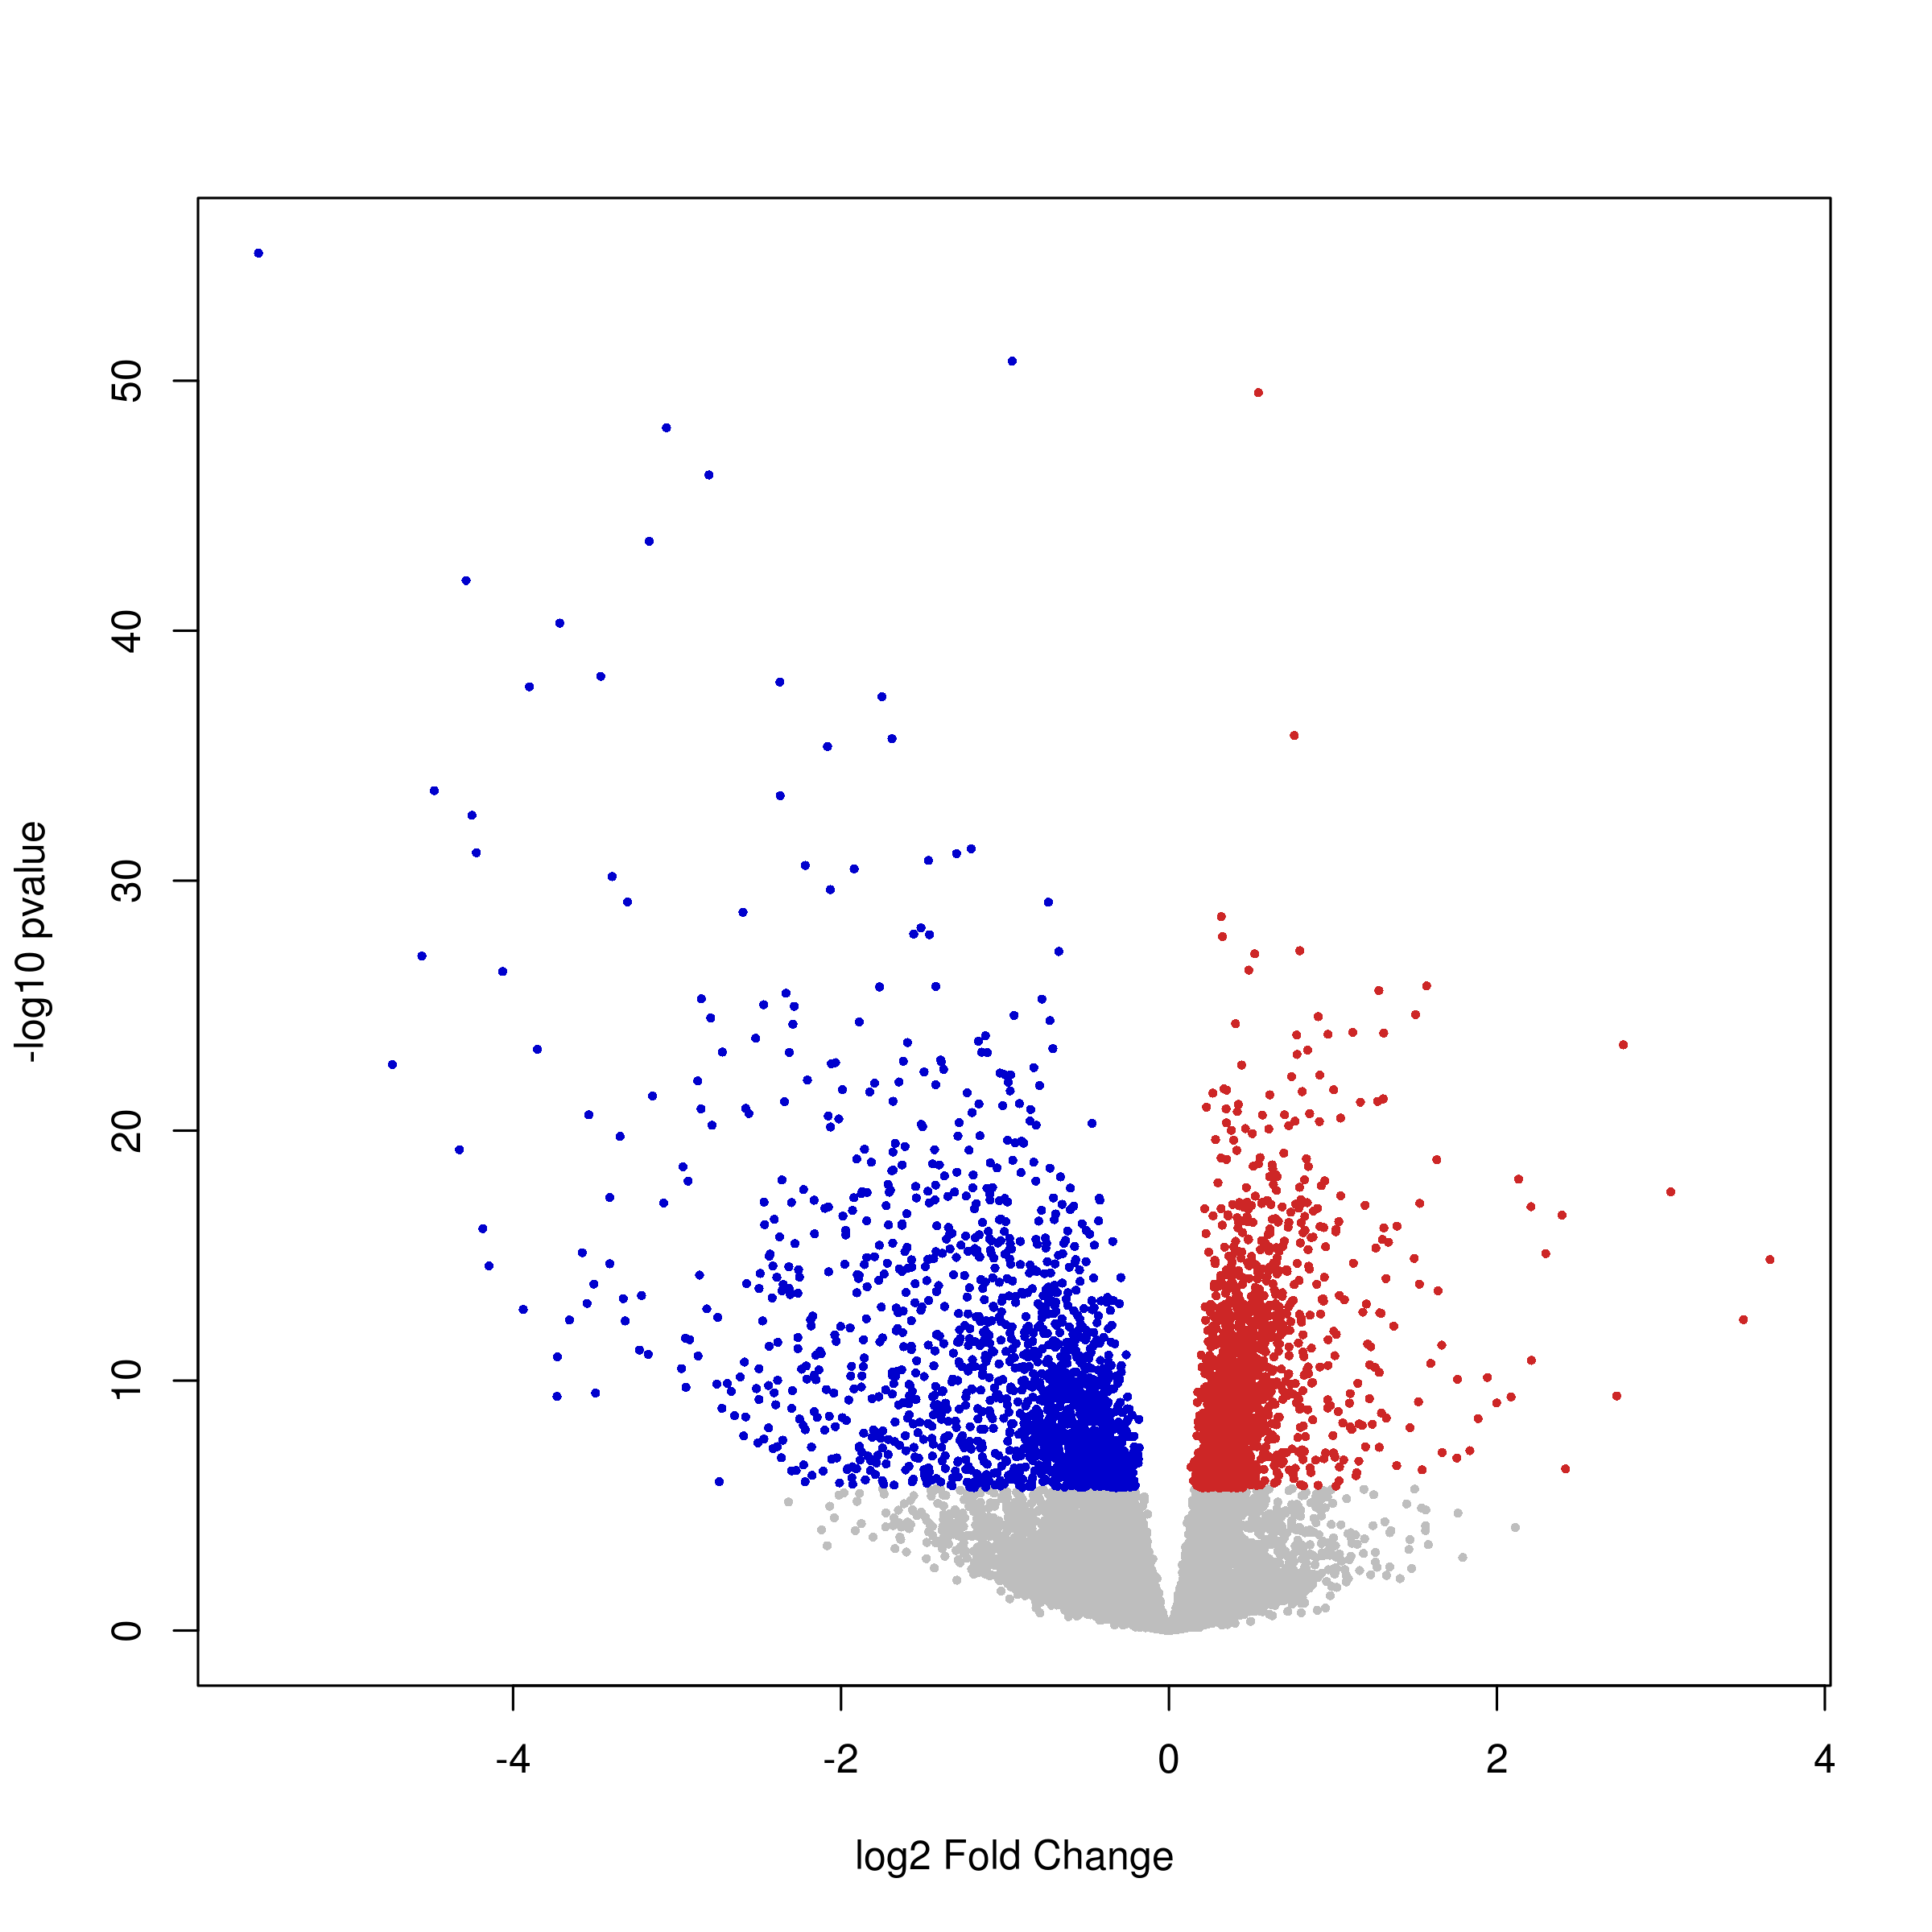
\includegraphics[width=0.45\textwidth]{environmental_risk/image/er_deseq_volcano.png}
	}
	\subfloat[Combining RNA Seq and microarray data\label{subfig2:combatVoc}]{%
		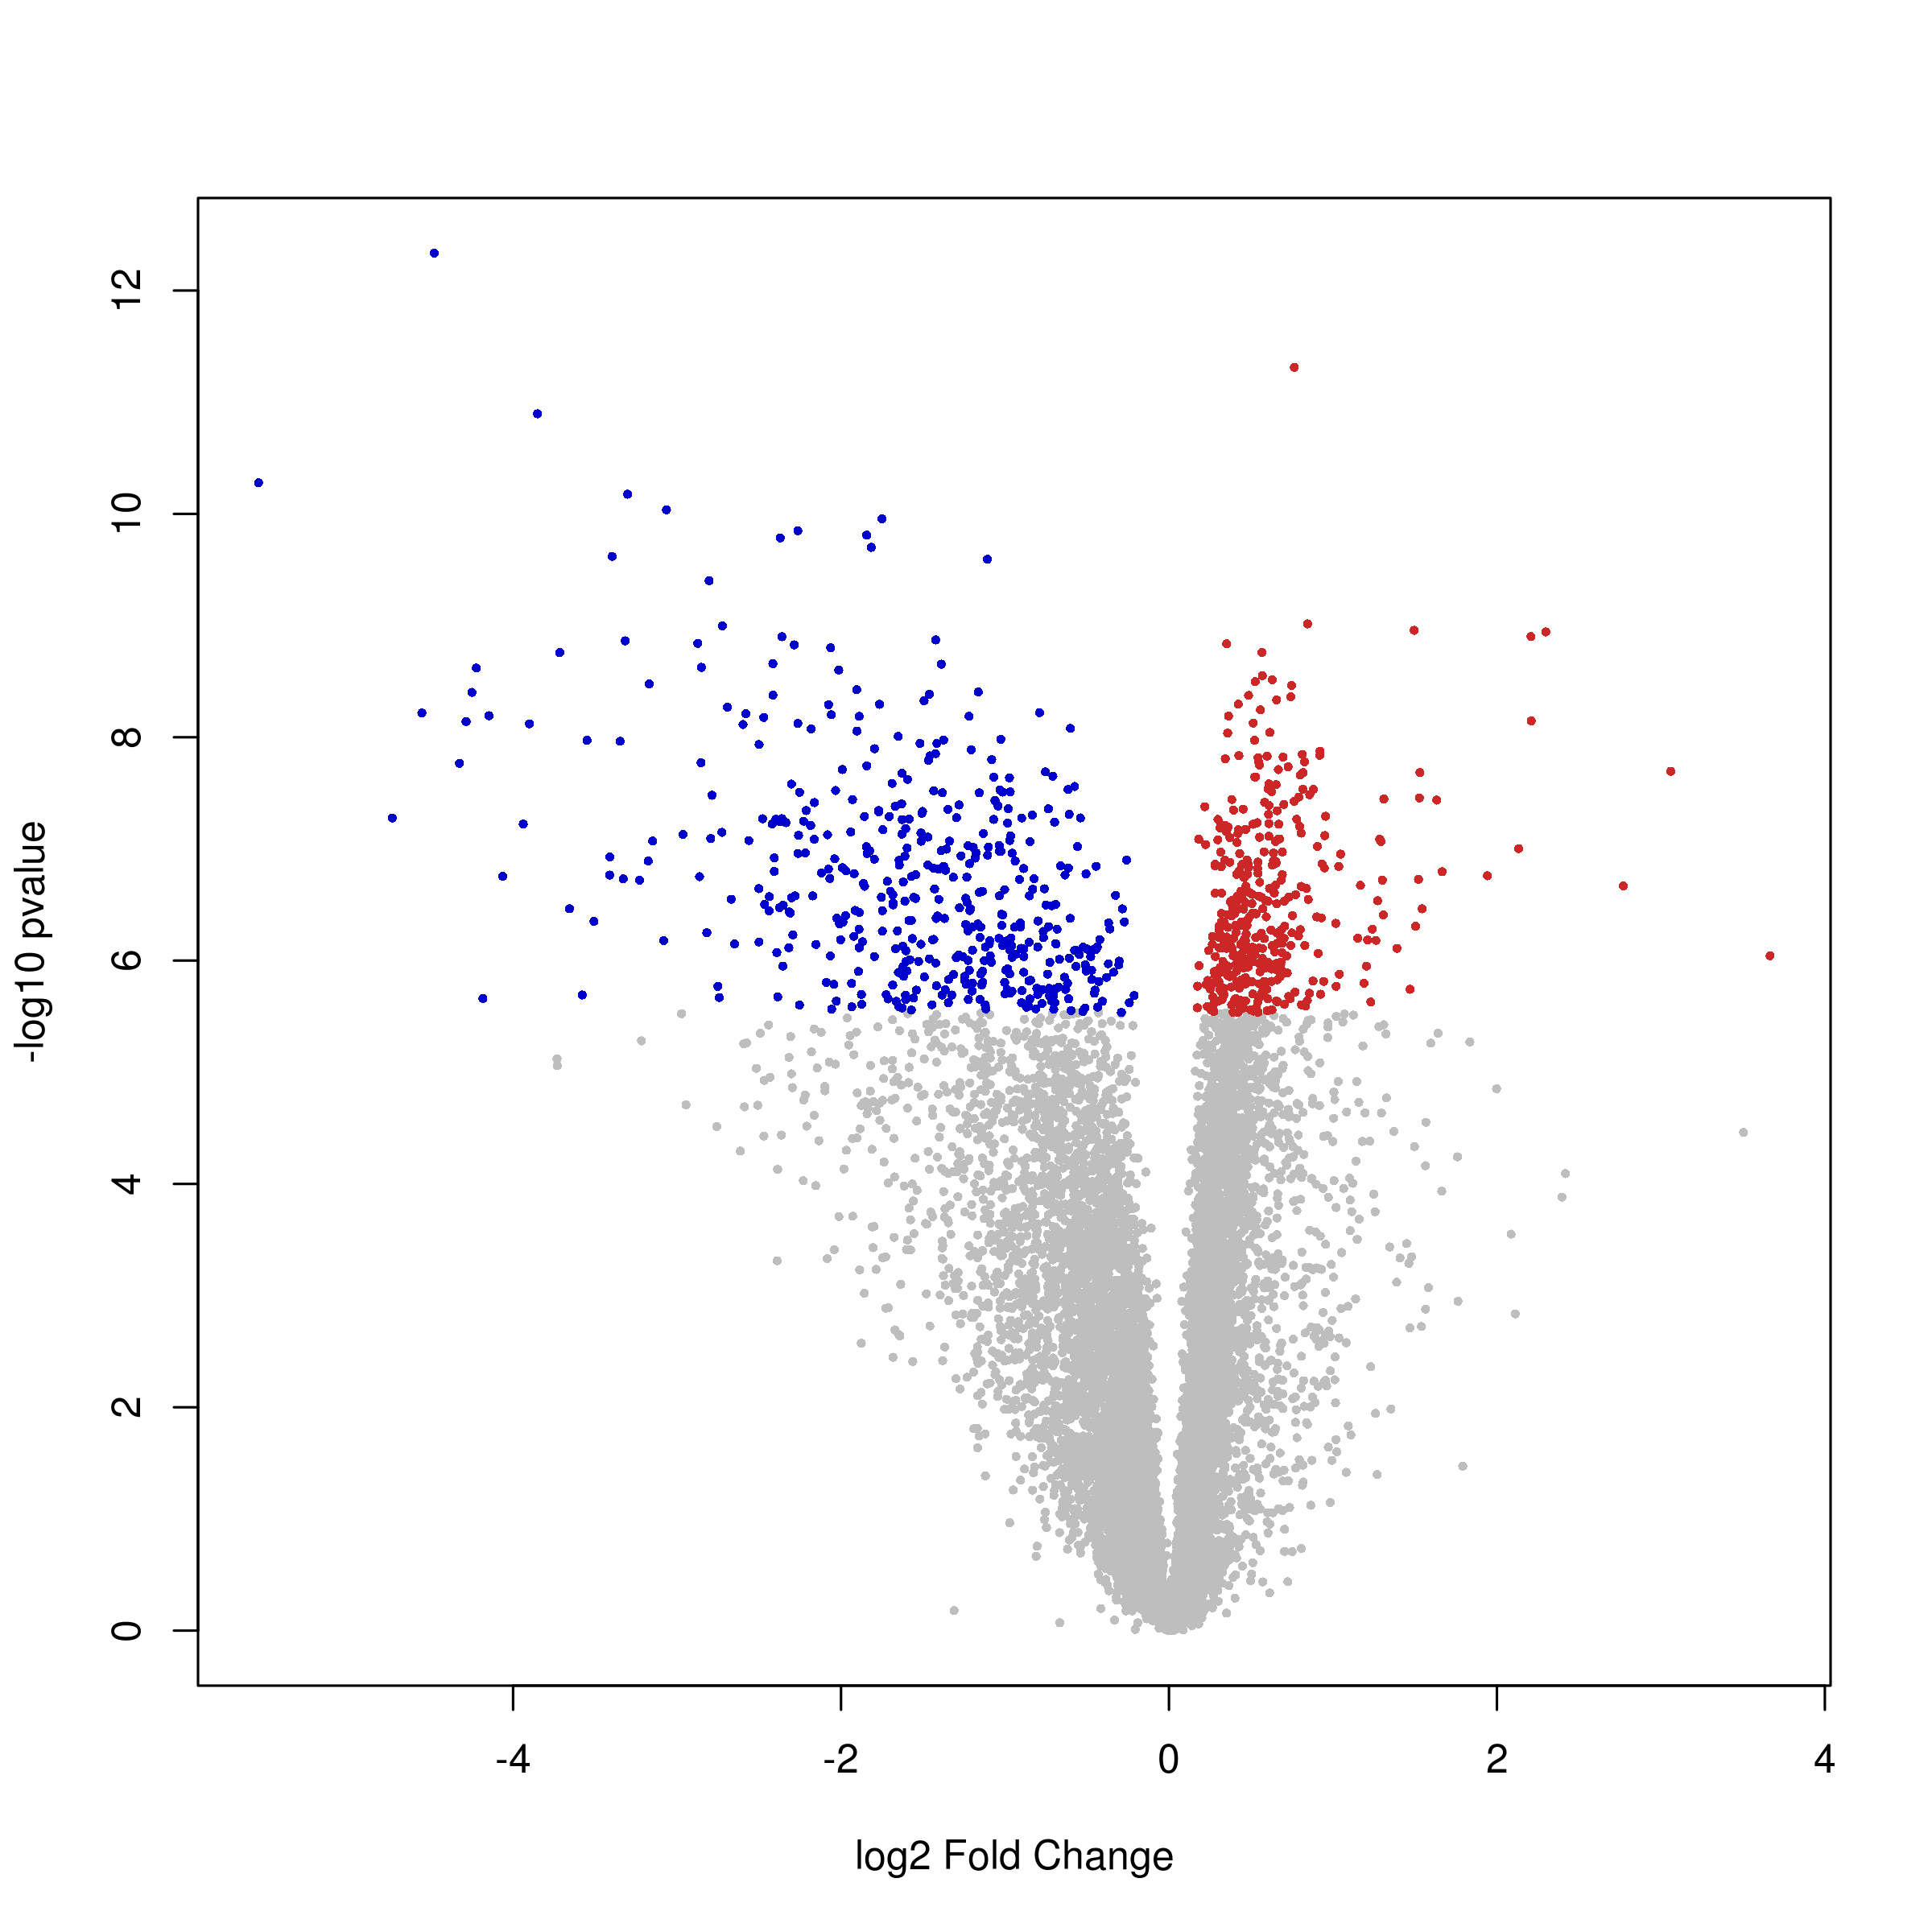
\includegraphics[width=0.45\textwidth]{environmental_risk/image/er_combat_volcano.png}
	}
	\caption[Volcano Plot]{Volcano plot of Case (PolyI:C) vs Control (Saline). 
		Genes that were significantly down-regulated are colored in blue whereas genes that were significantly up-regulated are colored in red. 
		a) Using only RNA-Seq data; 
		b) Using combination of RNA-Seq and microarray data.
	}
\end{figure}


\subsubsection{Gene Ontology(GO) enrichment}
A total of 28 GO terms were significantly overrepresented in the list of DEGs, with 10 and 18 GO terms represented by up- and down-regulated genes respectively, at a Bonferroni corrected p-value $<$ 0.05 (Table \ref{tab:geneOntologyFull}). 
Among the significant GO terms, a number of them, such as ``Developmental process'' (p-value $= 9.75\times 10^{-6}$), ``Regulation of neurogenesis'' (p-value $= 7.08\times 10^{-17}$) and ``Regulation of neurotransmitter levels'' (p-value $= 1.05\times 10^{-9}$) are related to brain function and development.

\subsubsection{Gene set enrichment}
Of the 149 gene sets tested, 27 were significantly enriched by the DEGs at a Bonferroni corrected p-value $<$ 0.05, including post-synaptic density protein and gene sets related to neurodevelopmental disorders, such as schizophrenia probable and autism associated modules (Table \ref{tab:fullGeneSetEnrichment}).

\subsection{Differential gene expression analysis with external controls}
We incorporated the external micro-array data as additional controls.
After quality control (QC), there are a total of 13,112 genes that can be found in both our RNA Seq data and the microarray chips.
Among the 13,112 genes, 868 were found to be differentially expressed (398 up-regulated and 470 down-regulated) with a Bonferroni-corrected p-value $<$ 0.05.
A volcano plot of PolyI:C versus Saline for all genes passing QC is presented in Figure \ref{subfig2:combatVoc}. 851 of the DEGs (98.0$\%$) overlapped with those discovered in our previous analysis without these external control data. 
Seven of the candidate schizophrenia genes previously identified by the PGC remained in our DEG list, including the GABA enzyme, \textit{Gad1} and \textit{Gad2}; \textit{Gabra3}, \textit{Ctnna2} and the dopamine-related gene, \textit{Th} (Table \ref{tab:candidateGeneTable}). 

\subsubsection{Gene Ontology enrichment}
The GO enrichment analysis found a total of 24 significantly enriched GO terms, of which 8 were enriched by the up-regulated genes and 16 were enriched by those down-regulated.
21 of them (87.5$\%$) overlapped with those found in the previous analysis without these external control data. ``Regulation of neurogenesis'' (enrichment p-value $= 4.94\times10^{-5}$) and ``Regulation of neurotransmitter levels'' (enrichment p-value $= 1.4\times10^{-7}$) were still among the enriched GO terms. 
\subsubsection{Gene set enrichment}
The gene-set enrichment analysis identified 5 enriched brain-related gene sets in the DEGs (Table \ref{tab:targetGeneSetEnrichment}), which were all identified in the previous analysis without these external control data. 
% Table generated by Excel2LaTeX from sheet 'Sheet1'
\afterpage{
\setlength\LTcapwidth{\textwidth}
\begin{longtable}{rrrrrr}
	\caption{Candidate genes for schizophrenia. We compared the candidate genes generated from the Psychiatric Genomic Consortium\cite{Greenwood2011} with the differentially expressed genes list from our study. It was found that majority (hyper geometric p-value $= 1.12\times 10^{-11}$) of the candidate genes were differentially expressed upon exposed to early maternal immune activation. Seven of the candidate genes remained in our differentially expressed gene list even after including the external control. Here only those that were significantly differentiated were shown}\label{tab:candidateGeneTable}\\
    \toprule
    \multicolumn{1}{c}{\multirow{2}[4]{*}{\textbf{Gene Name}}} & \multicolumn{3}{r}{Without external controls} &       & With external controls* \\
    \multicolumn{1}{c}{} & baseMean & Log2 Fold Change & Bonferroni Corrected P &       & Bonferroni Corrected P \\
    \midrule
    \textit{Adra2a} & 132.01 & -1.41 & $1.32\times 10^{-9}$ &       & 0.269 \\
    \textit{Adrbk2} & 400.52 & -0.343 & $1.77\times 10^{-3}$ &       & 1 \\
    \textit{Akt1} & 8537.11 & 0.0816 & 0.0364 &       & 1 \\
    \textit{Aspm} & 4875.21 & -0.179 & 0.017 &       & 1 \\
    \textit{Cacng2} & 30.78 & -1.53 & $1.21\times 10^{-8}$ &       & 0.233 \\
    \textit{Camk2a} & 357.99 & -0.583 & $6.25\times 10^{-8}$ &       & 1 \\
    \textit{Chrna4} & 844.89 & -0.278 & 0.0456 &       & 1 \\
    \textit{Chrnb2} & 336.29 & -1.1  & $7.66\times 10^{-11}$ &       & 0.0122 \\
    \textit{Crhr2} & 15.57 & 0.844 & 0.0146 &       & 1 \\
    \textit{Ctnna2} & 825.55 & -0.732 & $1.23\times 10^{-8}$ &       & 0.649 \\
    \textit{Dbh} & 31.55 & -2.49 & $5.15\times 10^{-15}$ &       & 0.0768 \\
    \textit{Dgcr2} & 3710.98 & 0.228 & $1.22\times 10^{-5}$ &       & 1 \\
    \textit{Disc1} & 54.78 & -0.58 & $1.05\times 10^{-3}$ &       & NA \\
    \textit{Dlg4} & 1626.55 & -0.353 & $2.45\times 10^{-11}$ &       & 0.0596 \\
    \textit{Drd2} & 12.38 & -0.974 & $7.79\times 10^{-3}$ &       & 1 \\
    \textit{Dtnbp1} & 1088.18 & 0.268 & $5.70\times 10^{-5}$ &       & 1 \\
    \textit{Ebf2} & 1003.45 & -0.451 & 0.025 &       & 1 \\
    \textit{Eea1} & 983.87 & -0.245 & $2.08\times 10^{-3}$ &       & 1 \\
    \textit{Erbb4} & 291.96 & -0.836 & $1.12\times 10^{-7}$ &       & 0.0912 \\
    \textit{Fez1} & 2783.05 & -0.581 & $4.68\times 10^{-11}$ &       & 1 \\
    \textit{Gabra3} & 204.37 & -0.634 & $1.67\times 10^{-8}$ &       & 0.00294 \\
    \textit{Gabrb2} & 150.74 & -1.137 & $4.73\times 10^{-17}$ &       & 0.0618 \\
    \textit{Gad1} & 80.15 & -2.96 & $2.79\times 10^{-19}$ &       & 0.00127 \\
    \textit{Gad2} & 183.28 & -1.66 & $1.25\times 10^{-13}$ &       & 0.0398 \\
    \textit{Grid2} & 15.99 & -0.933 & $2.76\times 10^{-3}$ &       & 1 \\
    \textit{Grik4} & 92.8  & -0.675 & $8.44\times 10^{-6}$ &       & 1 \\
    \textit{Grin3a} & 49.81 & -0.524 & $8.88\times 10^{-3}$ &       & 1 \\
    \textit{Grm2} & 250.43 & -0.673 & $3.66\times 10^{-4}$ &       & 1 \\
    \textit{Grm3} & 32.98 & -0.822 & $1.22\times 10^{-3}$ &       & 1 \\
    \textit{Grm4} & 164.28 & -0.659 & $7.32\times 10^{-5}$ &       & 1 \\
    \textit{Gsk3b} & 5068.93 & -0.197 & $6.37\times 10^{-4}$ &       & 1 \\
    \textit{Htr1b} & 121.93 & 0.448 & $9.74\times 10^{-4}$ &       & 1 \\
    \textit{Kcnh2} & 835.89 & -0.18 & 0.016 &       & 1 \\
    \textit{Ncam1} & 728.17 & -0.832 & $1.57\times 10^{-7}$ &       & 1 \\
    \textit{Nde1} & 6430.74 & 0.107 & $1.81\times 10^{-3}$ &       & 1 \\
    \textit{Ndel1} & 1195.39 & 0.114 & 0.0293 &       & 1 \\
    \textit{Nos1ap} & 109.8 & -0.579 & $3.86\times 10^{-5}$ &       & 1 \\
    \textit{Notch4} & 532.12 & -0.387 & $1.38\times 10^{-5}$ &       & 1 \\
    \textit{Ppp3cc} & 120.61 & -0.485 & $4.38\times 10^{-5}$ &       & 1 \\
    \textit{Prodh} & 550.47 & 0.699 & $7.59\times 10^{-13}$ &       & 0.807 \\
    \textit{Rgs4} & 164.1 & -0.958 & 0.0127 &       & 1 \\
    \textit{Slc1a2} & 777.36 & -1.28 & $4.82\times 10^{-21}$ &       & $6.92\times 10^{-3}$ \\
    \textit{Slc32a1} & 44.4  & -4.56 & $1.03\times 10^{-27}$ &       & $1.04\times 10^{-3}$ \\
    \textit{Slc6a1} & 126.37 & -1.88 & $3.32\times 10^{-18}$ &       & 0.341 \\
    \textit{Slc6a4} & 15.86 & -1.12 & $5.41\times 10^{-3}$ &       & 1 \\
    \textit{Sp4} & 910.49 & -0.407 & $4.15\times 10^{-11}$ &       & 0.063 \\
    \textit{Th} & 87.29 & -2.16 & $1.34\times 10^{-16}$ &       & $6.59\times 10^{-3}$ \\
    \textit{Ywhae} & 36516.86 & 0.258 & $1.32\times 10^{-6}$ &       & 1 \\
    \bottomrule
    \multicolumn{6}{l}{* Genes not found in the external control data were marked with NA} \\
    
\end{longtable}%
}

% Table generated by Excel2LaTeX from sheet 'Sheet2'
\afterpage{
\begin{landscape}
\setlength\LTcapwidth{\textwidth}
\begin{longtable}{cp{3cm}cccccp{5cm}}
  \caption{Gene Ontology(GO) enrichment Result. GOrilla and REViGO were used to perform GO enrichment analysis. Similar GO terms were clustered together and represented by a single representative GO terms. Here, only the representative GO terms were shown. }\label{tab:geneOntologyFull}\\
    \toprule
    \multicolumn{1}{c}{} & \multicolumn{3}{r}{\textit{\textbf{RNA-seq gene level}}} &  & \multicolumn{3}{r}{\textit{\textbf{Microarray and RNA-seq combined}}} \\
    \midrule
    \multicolumn{1}{c}{} & \multicolumn{3}{r}{\textit{\textbf{GO functional enrichment}}} & \textit{\textbf{}} & \multicolumn{3}{r}{\textit{\textbf{GO functional enrichment}}} \\
    \textit{\textbf{GO ID}} & \textit{\textbf{GO term}} & \textit{\textbf{P-value}} & \textit{\textbf{Direction}} & \textit{\textbf{}} & \textit{\textbf{Minimum P-value}} & \textit{\textbf{Direction}} & \textit{\textbf{Represented by}} \\
    GO:0007610 & behavior & $9.67\times 10^{-19}$ & Down  &       & $6.76\times 10^{-8}$ & Down & defense response \\
    GO:0022610 & biological adhesion & $4.65\times 10^{-10}$ & Down  &       & $8.66\times 10^{-5}$ & Down  &  \\
    GO:0065007 & biological regulation & $2.15\times 10^{-18}$ & Down  &       & $1.97\times 10^{-8}$ & Down  &  \\
    GO:0001775 & cell activation & $5.56\times 10^{-7}$ & Down  &       & $4.96\times 10^{-10}$ & Down  &  \\
    GO:0007155 & cell adhesion & $6.12\times 10^{-10}$ & Down  &       & $7.97\times 10^{-5}$ & Down  &  \\
    GO:0007049 & cell cycle & $9.99\times 10^{-3}$ & Up    &       & -     & -     &  \\
    GO:0008283 & cell proliferation & $5.53\times 10^{-3}$ & Up    &       & $1.83\times 10^{-3}$ & Up    &  \\
    GO:0008037 & cell recognition & $6.05\times 10^{-3}$ & Down  &       & $5.28\times 10^{-3}$ & Down  &  \\
    GO:0007267 & cell-cell signaling & $5.9\times 10^{-6}$ & Down  &       & -     & -     &  \\
    GO:0006928 & cellular component movement & $1.40\times 10^{-7}$ & Down  &       & $1.74\times 10^{-5}$ & Down  &  \\
    GO:0071840 & cellular component organization or biogenesis & $4.01\times 10^{-6}$ & Up    &       & -     & -     &  \\
    GO:0009987 & cellular process & $9.23\times 10^{-13}$ & Up    &       & $1.57\times 10^{-3}$ & Up    &  \\
    GO:0006974 & cellular response to DNA damage stimulus & $4.76\times 10^{-3}$ & Up    &       & -     & -     &  \\
    GO:0032502 & developmental process & $1.23\times 10^{-5}$ & Down  &       & -     & -     &  \\
    GO:0002376 & immune system process & $1.16\times 10^{-8}$ & Down  &       & $4.39\times 10^{-11}$ & Down  &  \\
    GO:0051703 & intraspecies interaction between organisms & $1.48\times 10^{-3}$ & Down  &       & -     & -     &  \\
    GO:0040011 & locomotion & $2.10\times 10^{-9}$ & Down  &       & $7.23\times 10^{-6}$ & Down  &  \\
    GO:1903047 & mitotic cell cycle process & $1.94\times 10^{-3}$ & Up    &       & -     & -     &  \\
    GO:0032501 & multicellular organismal process & $1.61\times 10^{-11}$ & Down  &       & -     & -     &  \\
    GO:0051704 & multi-organism process & $6.29\times 10^{-3}$ & Down  &       & -     & -     &  \\
    GO:0001890 & placenta development & $9.63\times 10^{-5}$ & Up    &       & $4.01\times 10^{-5}$ & Up    & osteoblast differentiation \\
    GO:0042391 & regulation of membrane potential & $1.79\times 10^{-9}$ & Down  &       & $1.40\times 10^{-7}$ & Down  & regulation of neurotransmitter levels \\
    GO:0050767 & regulation of neurogenesis & $3.54\times 10^{-17}$ & Down  &       & $6.82\times 10^{-11}$ & Down  & cell projection organization, cognition, immune effector process, regulation of multicellular organismal process \\
    \multicolumn{1}{c}{GO:0022613} & ribonucleoprotein complex biogenesis & \multicolumn{1}{c}{$1.02\times 10^{-27}$} & \multicolumn{1}{c}{Up} & \multicolumn{1}{c}{} & \multicolumn{1}{c}{$6.37\times 10^{-13}$} & \multicolumn{1}{c}{Up} &  \\
    \multicolumn{1}{c}{GO:0006396} & RNA processing & \multicolumn{1}{c}{$2.25\times 10^{-50}$} & \multicolumn{1}{c}{Up} & \multicolumn{1}{c}{} & \multicolumn{1}{c}{$5.18\times 10^{-15}$} & \multicolumn{1}{c}{Up} & translation \\
    \multicolumn{1}{c}{GO:0050658} & RNA transport & \multicolumn{1}{c}{$3.21\times 10^{-10}$} & \multicolumn{1}{c}{Up} & \multicolumn{1}{c}{} & \multicolumn{1}{c}{$1.17\times 10^{-3}$} & \multicolumn{1}{c}{Up} &  \\
    \multicolumn{1}{c}{GO:0023052} & signaling & \multicolumn{1}{c}{$4.36\times 10^{-9}$} & \multicolumn{1}{c}{Down} & \multicolumn{1}{c}{} & \multicolumn{1}{c}{-} & \multicolumn{1}{c}{-} &  \\
    \multicolumn{1}{c}{GO:0071353} & cellular response to interleukin-4 & \multicolumn{1}{c}{-} & \multicolumn{1}{c}{-} & \multicolumn{1}{c}{} & \multicolumn{1}{c}{$2.20\times 10^{-5}$} & \multicolumn{1}{c}{Up} &  \\
    \multicolumn{1}{c}{GO:0000082} & G1/S transition of mitotic cell cycle & \multicolumn{1}{c}{-} & \multicolumn{1}{c}{-} & \multicolumn{1}{c}{} & \multicolumn{1}{c}{$6.14\times 10^{-3}$} & \multicolumn{1}{c}{Up} &  \\
    \multicolumn{1}{c}{GO:0030001} & metal ion transport & \multicolumn{1}{c}{-} & \multicolumn{1}{c}{-} & \multicolumn{1}{c}{} & \multicolumn{1}{c}{$1.25\times 10^{-7}$} & \multicolumn{1}{c}{Down} &  \\
    \multicolumn{1}{c}{GO:0050896} & response to stimulus & \multicolumn{1}{c}{-} & \multicolumn{1}{c}{-} & \multicolumn{1}{c}{} & \multicolumn{1}{c}{$9.89\times 10^{-7}$} & \multicolumn{1}{c}{Down} &  \\
    \bottomrule
    \end{longtable}%
    
\end{landscape}
}
% Table generated by Excel2LaTeX from sheet 'Sheet3'
\begin{landscape}
\begin{table}[htbp]
  \centering
  \caption{Gene set enrichment results of differential expressed genes combining microarray and RNA Seq data.
  Enrichment results mapping to \textit{de-novo} mutations and common variants are also shown.
  It was noted that the Post-synaptic density protein (PSD) gene sets were enriched with \textit{de-novo} mutations from 3 out of 4 studies and only the microglia gene set was enriched by the common variants observed in the schizophrenia Genome-wide association study (GWAS) conducted by the Psychiatric Genomic Consortium\cite{Ripke2013}.}
    \begin{tabular}{cccccccc}
    \multicolumn{1}{c}{\multirow{3}[3]{*}{\textbf{Gene Set}}} & \multicolumn{1}{c}{\multirow{3}[3]{*}{\textbf{RNA Seq}}} & \textbf{Denovo } & \textbf{} & \textbf{} & \textbf{} & \textbf{GWAS} & \textbf{} \\
    \cline{3-8}
    
    \multicolumn{1}{c}{} & \multicolumn{1}{c}{} & 
    \multicolumn{1}{p{2.3cm}}{\multirow{2}[2]{*}{\textbf{Fromer et al.}}} & \multicolumn{1}{p{2cm}}{\multirow{2}[2]{*}{\textbf{Neale et al.}}} & \multicolumn{1}{p{2.4cm}}{\multirow{2}[2]{*}{\textbf{Sanders et al.}}} & \multicolumn{1}{p{2.3cm}}{\multirow{2}[2]{*}{\textbf{O'Roak et al.}}} & \multicolumn{1}{p{2.3cm}}{\multirow{2}[2]{*}{\textbf{Anney et al.}}} & \multicolumn{1}{p{2.3cm}}{\multirow{2}[2]{*}{\textbf{Ripke et al.}}} \\[0.25cm]
    \multicolumn{1}{c}{} & \multicolumn{1}{c}{} & \multicolumn{1}{c}{\textbf{Scz\cite{Fromer2014}}} & \multicolumn{1}{c}{\textbf{ASD\cite{Neale2012}}} & \multicolumn{1}{c}{\textbf{ASD\cite{Sanders2012}}} & \multicolumn{1}{c}{\textbf{ASD\cite{ORoak2012}}} & \multicolumn{1}{c}{\textbf{ASD\cite{Anney2010a}}} & \multicolumn{1}{c}{\textbf{Scz\cite{Ripke2013}}} \\
    \midrule
    Neuron definite\cite{Cahoy2008} & $2.66\times 10^{-4}$ & 0.358 & 0.381 & 1     & $3.83\times10^{-3}$ & 0.614 & 0.188 \\
    Neuron probable\cite{Cahoy2008} & $5.77\times10^{-3}$ & $7.14\times10^{-9}$ & 0.373 & 1     & $2.51\times10^{-7}$ & 0.763 & 0.323 \\
    Microglia (Type1)\cite{Miller2010} & $3.17\times10^{-8}$ & 1     & 1     & 1     & 1     & 0.938 & $9.64\times10^{-3}$ \\
    PSD proteins\cite{Bayes2011} & $3.54\times10^{-5}$ & $3.07\times10^{-10}$ & 0.0732 & $2.63\times10^{-3}$ & $3.35\times10^{-4}$ & 0.461 & 0.548 \\
    Ribosome\cite{Miller2010} & $9.41\times10^{-4}$ & 1     & 1     & 1     & 1     & 0.489 & 0.317 \\
    \bottomrule
    \end{tabular}%
  \label{tab:targetGeneSetEnrichment}%
\end{table}%
\end{landscape}


\begin{figure}
	\caption[rtPCR Results]{real time PCR validation of RNA Seq results.
		The delta CT values are highly correlated with the RNA-Seq counts (case: pearson correlation = -0.968, control: pearson correlation = 0.952), suggesting that the RNA-Seq count is a true representation of the RNA concentration.
		The difference in detla CT between the cases and controls also support the differential gene expression results of the RNA Sequencing analysis.}\label{fig:rtResult}
		\vspace{-20pt}
	\begin{center}
		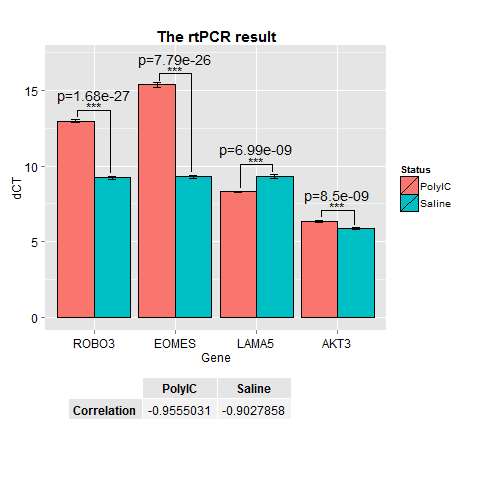
\includegraphics[trim=0cm 2cm 0cm 1cm, clip=true, width=0.7\textwidth]{environmental_risk/image/er_rtPCR.png}
	\end{center}
\end{figure}

\subsection{Test for burden of genetic risk variants in enriched brain-related gene sets in schizophrenia and autism cohorts }
Among the 27 enriched brain-related gene sets identified in the analysis without external control (Table \ref{tab:fullGeneSetEnrichment}), three (``Post-synaptic Density Proteins'', ``Neuron Probable'' and ``Down with Alzheimer's'') were enriched with rare \textit{de-novo} mutations in more than one study. 
In addition, the ``Oligodendrocyte Marker'' gene set was enriched with both rare \textit{de-novo} mutations and common genetic variants in schizophrenia studies. 

When combined with external control, only 5 gene sets remained \ref{tab:targetGeneSetEnrichment}. 
Of the 5 remaining gene sets, only the microglia gene set from \citet{Miller2010} was found to contain significantly more common genetic variations associated with schizophrenia in the PGC genome wide association study (GWAS).
Whereas the significant ``Neuron Probable'' and ``Post-synaptic Density Proteins'' were among the 5 remaining gene sets.

\subsection{RT-PCR validation of RNA-Seq data}
The CT value is the unit used during rtPCR to indicates the mRNA concentration.
A high CT value means more PCR cycle is required to detect the mRNA, therefore indicating a low mRNA concentration.
Thus, a high CT value represent a low mRNA concentration and a low CT value represent a high mRNA concentration, as oppose to the RNA Seq count value.

In the rtPCR, the CT values were highly negatively correlated with the RNA-Seq (Case: r  = -0.968, p = $2.98\times10^{-15}$; Control: r  = -0.952, p= $2.834\times10^{-13}$), suggesting that the RNA-Seq counts truly reflected the true mRNA concentration (Figure \ref{fig:rtResult}). 
Simple T-test performed on the relative CT values confirmed that all genes tested were significantly differentially expressed (Figure \ref{fig:rtResult}).


	
\subsection{Alternative splicing}
\subsection{De-novo Assembly}

\section{Discussion}
In this pilot study, we found that maternal immune activation (MIA) triggers significant gene expression differences in the embryonic brain. 
These results also contribute Proof of Concept evidence that exposure to MIA in early gestation impacts upon genes implicated in neurodevelopmental conditions such as schizophrenia and autism. 

\subsection{MIA acts upon genes necessary for synaptic structure and function}
We discovered that GABA- and glutamate- related genes such as \textit{Gad1}, \textit{Gad2}, \textit{Gabra3}, \textit{Slc32a1} and \textit{Slc1a2} were significantly down-regulated following MIA; and most of the differentially expressed genes (DEGs) were functionally related to neurogenesis and neurotransmitter regulation.
Glutamate and GABA are known to play critical roles in neurogenesis, neuronal migration and synaptogenesis during development\cite{Cameron1998,LaMantia1995,LoTurco1995} and disruption of the GABAergic and glutamatergic systems leading to excitation/inhibition imbalance has been implicated in neurodevelopmental psychiatric disorders, such as schizophrenia\cite{Wassef2003} and autism\cite{Rubenstein2003}.

For example, the expression of \textit{Dlg4} (discs, large homolog 4), also known as postsynaptic density protein 95 (\textit{PSD95})\cite{DeBartolomeis2014}, was significantly lower in the PolyI:C-exposed fetal brains. 
\textit{PSD95} is a critical regulator of the neurexin-neuroligin-SHANK pathway implicated in autism spectrum disorders\cite{Feyder2010}.
\textit{PSD95} abnormalities are therefore thought to alter the balance of excitation and inhibition, and variations in this balance might change, not only local circuit function, but also connectivity patterns between brain regions, leading to developmental and behavioral deficits\cite{Cline2005}. 
Consistent with this, \textit{PSD95} have been associated with autism\cite{Risch1999} and schizophrenia\cite{Hahn2006}. 

\subsection{MIA acts on microglial/inflammatory genes}
The genes influenced by MIA included multiple microglia markers such as \textit{Cx3cr1} (chemokine receptor 1) and \textit{Csf1r} (colony stimulating factor 1 receptor) which were both down-regulated in the PolyI:C-exposed fetal brain. 
Microglia are the resident macrophages of the brain and the first and main form of active immune response within the central nervous system (CNS).
One of the main functions of microglia in brain development is synaptic pruning\cite{Paolicelli2011}, and thus deregulation of microglia might be expected to have a prolonged effect on brain development. 
Indeed, a recent study of the chemokine receptor \textit{Cx3cr1} knock out mouse found that a decrease in microglia was associated with a decrease in synaptic multiplicity and also autism-like behaviors such as increased repetitive behaviors and impaired social interactions\cite{Rogers2011}. 
\citet{Erblich2011} also reported enlarged lateral ventricles and reduced volume of olfactory area without changes of overall brain volume in the microglia marker \textit{Csf1r} knock-out mice, which is similar to our previous findings in the MIA mouse model\cite{Li2009c}. 
%If there isn't enough pages, we can elaborate here
Thus a similar \textit{Csf1r} deficit might be acting in both models of neurodevelopmental disorder.
	
\subsection{Overview}
Synaptic and microglial mechanisms are not independent and it is increasingly recognized that brain excitatory-inhibitory balance is a product of interplay between neuronal and glial systems\cite{Zhan2014}. 
Moreover, neurodevelopmental disorders are increasingly understood to be influenced by synaptic and/or neuroinflammatory pathology and this complexity likely maps to the heterogeneous nature of these conditions\cite{Garay2010}.

\subsection{Limitations}
%This has to be more detail analysis of the study. cannot be the same as the one in the paper
We first acknowledge that the sample size of current study is modest. 
That said, the effect sizes observed were large and multimodal measures acquired from the same animals were consistent with predictions. 
Second, we examined only male fetal brains in the current study. 
The decision to direct experimental resources to males was made because males with neurodevelopmental disorders such as autism out-number females; and there is evidence that the male fetus is more vulnerable to environmental exposures such as inflammation in prenatal life\cite{Bergeron2013}\cite{Lein2007}. 



\section{Conclusion}
Short conclusion on the Environmental Risk.
Also link the result to the next chapter.

	\chapter[Genetic Risk Factor - Heritability Estimation]{Genetic Risk Factor:\\Heritability Estimation}
		\section{Estimation of Heritability}
			\subsection{Estimating the Mean}
			\subsection{Estimating the Variance}
			To calculate the variance of the estimation, we will need to obtain the variance covariance matrix of $h$. 
			Because $\boldsymbol{h}=\boldsymbol{(\rho^2)^{-1}f}$, we can obtain the variance covariance matrix of $h$ as
			$$
			\boldsymbol{\mathrm{Cov}(h)} = \boldsymbol{(\rho^2)^{-1}\mathrm{Cov}(f)(\rho^2)^{-1}}
			$$
			As $f$ is a function of $\chi^2$, we can obtain the variance covariance matrix of $f$ by first calculating the variance covariance matrix of the $\chi^2$ variables.
			
			First, let that $\chi_i$ be the standardized genotype with standard normal mean $z_i$ and non-centrality parameter $\mu_i$, we have
			\begin{align*}
			\mathrm{E}[\chi_i]&=\mathrm{E}[z_i+\mu_i]\\
			&=\mu_i\\
			\mathrm{Var}(\chi_i) &=\mathrm{E}[(z_i+\mu_i)^2]+\mathrm{E}[(z_i+\mu_i)]^2\\
			&=\mathrm{E}[z_i^2+\mu_i^2+2z_i\mu_i]+\mu_i^2\\
			&=1
			\end{align*}
			Given the LD between two genotype $\chi_i$ and $\chi_j$ are $\rho_{ij}$, then
			\begin{align*}
			\mathrm{Cov}(\chi_i,\chi_j)&=\mathrm{E}[(z_i+\mu_i)(z_j+\mu_j)]-\mathrm{E}[z_i+\mu_i]\mathrm{E}[z_j+\mu_j]\\
			&=\mathrm{E}[z_iz_j+z_i\mu_j+\mu_iz_j+\mu_i\mu_j]-\mu_i\mu_j\\
			&=\mathrm{E}[z_iz_j]+\mathrm{E}[z_i\mu_j]+\mathrm{E}[z_j\mu_i]+\mathrm{E}[\mu_i\mu_j]-\mu_i\mu_j\\
			&=\mathrm{E}[z_iz_j]
			\end{align*}
			As the genotypes are standardized, therefore $\mathrm{Cov}(\chi_i,\chi_j)==\mathrm{Cor}(\chi_i,\chi_j)$ and we can obtain
			$$
				\mathrm{Cov}(\chi_i,\chi_j)=\mathrm{E}[z_iz_j]=\rho_{ij}
			$$
			Given these information, we can then calculate $\mathrm{Cov}(\chi_i^2,\chi_j^2)$ as:
			\begin{align*}
				\mathrm{Cov}(\chi_i^2,\chi_j^2)&=\mathrm{E}[(z_i+\mu_i)^2(z_j+\mu_j)^2]-\mathrm{E}[z_i+\mu_i]\mathrm{E}[z_j+\mu_j]\\
				&=\mathrm{E}[(z_i^2+\mu_i^2+2z_i\mu_i)(z_j^2+\mu_j^2+2z_j\mu_j)]-\mathrm{E}[z_i^2+\mu_i^2+2z_i\mu_i]\mathrm{E}[z_j^2+\mu_j^2+2z_j\mu_j]\\
				&=\mathrm{E}[(z_i^2+\mu_i^2+2z_i\mu_i)(z_j^2+\mu_j^2+2z_j\mu_j)]-(\mathrm{E}[z_i^2]+\mathrm{E}[\mu_i^2]+2\mathrm{E}[z_i\mu_i])(\mathrm{E}[z_j^2]+\mathrm{E}[\mu_j^2]+2\mathrm{E}[z_j\mu_j])\\
				&=\mathrm{E}[z_i^2(z_j^2+\mu_j^2+2z_j\mu_j)+\mu_i^2(z_j^2+\mu_j^2+2z_j\mu_j)+2z_i\mu_i(z_j^2+\mu_j^2+2z_j\mu_j)]-(1+\mu_i^2)(1+\mu_j^2)\\
				&=\mathrm{E}[z_i^2(z_j^2+\mu_j^2+2z_j\mu_j)]+\mu_i^2\mathrm{E}[z_j^2+\mu_j^2+2z_j\mu_j]+2\mu_i\mathrm{E}[z_i(z_j^2+\mu_j^2+2z_j\mu_j)]-(1+\mu_i^2)(1+\mu_j^2)\\
				&=\mathrm{E}[z_i^2z_j^2+z_i^2\mu_j^2+2z_i^2z_j\mu_j]+\mu_i^2+\mu_i^2\mu_j^2+2\mu_i\mathrm{E}[z_iz_j^2+z_i\mu_j^2+2z_iz_j\mu_j]-(1+\mu_i^2)(1+\mu_j^2)\\
				&=\mathrm{E}[z_i^2z_j^2]+\mu_j^2+\mu_i^2+\mu_i^2\mu_j^2+4\mu_i\mu_j\mathrm{E}[z_iz_j]-(1+\mu_i^2+\mu_j^2+\mu_i\mu_j)\\
				&=\mathrm{E}[z_i^2z_j^2]+4\mu_i\mu_j\mathrm{E}[z_iz_j]-1
			\end{align*}
			Remember that $\mathrm{E}[z_iz_j] = \rho_{ij}$, we then have
			$$
			\mathrm{Cov}(\chi_i^2, \chi_j^2)=\mathrm{E}[z_i^2z_j^2]+4\mu_i\mu_j\rho_{ij}-1
			$$
			By definition, 
			$$
				z_i|z_j\sim N(\mu_i+\rho_{ij}(z_j-\mu_j),1-\rho_{ij}^2)
			$$
			We can then calculate $\mathrm{E}[z_i^2z_j^2]$ as
			\begin{align*}
				\mathrm{E}[z_i^2z_j^2]&=\mathrm{Var}[z_iz_j]+\mathrm{E}[z_iz_j]^2\\
				&=\mathrm{E}[\mathrm{Var}(z_iz_j|z_i)]+\mathrm{Var}[\mathrm{E}[z_iz_j|z_i]]+\rho_{ij}^2\\
				&=\mathrm{E}[z_j^2\mathrm{Var}(z_i|z_j)]+\mathrm{Var}[z_j\mathrm{E}[z_i|z_j]]+\rho_{ij}^2\\
				&=(1-\rho_{ij}^2)\mathrm{E}[z_j^2]+\mathrm{Var}(z_j(\mu_i+\rho_{ij}(z_j-\mu_j)))+\rho_{ij}^2\\
				&=(1-\rho_{ij}^2)+\mathrm{Var}(z_j\mu_i+\rho_{ij}z_j^2-\mu_jz_j\rho_{ij})+\rho_{ij}^2\\
				&=1+\mu_i^2\mathrm{Var}(z_j)+\rho_{ij}^2\mathrm{Var}(z_j^2)-\mu_j^2\rho_{ij}^2\mathrm{Var}(z_j)\\
				&=1+2\rho_{ij}^2
			\end{align*}
			As a result, the variance covariance matrix of the $\chi^2$ variances can be calculated as
			$$
				\mathrm{Cov}(\chi_i^2,\chi_j^2) = 2\rho_{ij}^2+4\rho_{ij}\mu_i\mu_j
			$$

			Now that we have calculated the variance covariance matrix of $\chi^2$, we can get the variance covariance matrix of $f$ as
			\begin{align*}
			Cov(f_i,f_j) &= \frac{d}{d(\chi_i^2)}\frac{\chi_i^2-1}{n-2+\chi_i^2}\frac{d}{d(\chi_j^2)}\frac{\chi_j^2-1}{n-2+\chi_j^2}Cov(\chi_i^2,\chi_j^2) \\
			&= \frac{(n-1)^2}{(n-2+\chi_i^2)^2(n-2+\chi_j^2)^2}Cov(\chi_i^2,\chi_j^2)
			\end{align*}
		\section{Simulation Study}
		\nomenclature{CEU}{Utah residents with Northern and Western European ancestry from the CEPH collection} 
			\subsection{Quantitative Trait}
			\subsection{Case-Control Study design}
		\section{Result}
		\section{Discussion}
		\section{Conclusion}

	\chapter[Genetic Risk Factor - Risk Prediction]{Genetic Risk Factor:\\ Risk Prediction}
		\section{Risk Estimation}
		\section{Simulation Study}
		\section{Result}
		\section{Conclusion}

%\chapter{General Introduction and literature review (What has been done)}

\section{Neurodevelopmental disorders}
\subsection{Schizophrenia}
\subsection{Autism}

To understand these disorders, researchers conduct different studies
\section{Contribution of Genetic and Environmental risk factors}
\subsection{Epidemiological studies}
Looking into records
Find out what is common between the people
e.g. alcohol use, prenatal infection

Here we will discuss how different environmental risk factors were considered as risk factors for neurodevelopmental disorders (e.g. Etiological studies)
\subsection{Postnatal stress}
\subsection{Maternal use of alcohol}
\subsection{Socio-economical status}
\subsection{Age of parents}
\subsection{Maternal immune activation}
At the end, we would like to comparing different environmental risk factors and then say that maternal immune activation were the most interested as this is the single biggest risk factor

\subsection{Twin Studies}
Only small amount of similarity between the environmental factors
Will there be anything other than environment?
Use twins studies to find out.

\section{Genetic Risk Factors}
Now we know genetic is the main factor, how to study it?
And also how people study the role of genetics in a disease.
So basically, will have brief discussion on gwas, exome sequencing and whole genome sequencing
\subsection{Common Single Nucleotide Polymorphism}
\subsubsection{Genome-wide association studies}
\subsection{Rare Single Nucleotide Mutation}
\subsection{Copy Number Variation (CNV)}

\section{Aim of the study}
\paragraph{} In this thesis


%\chapter{Genetic risk factors of Neurodevelopmental disorders}
\section{Introduction}
\subsection{Heritability estimate}
\subsubsection{Heritability explained by Common SNPs}
\subsubsection{Missing Heritability}
\subsubsection{Risk Prediction}
\subsection{Challenge of heritability estimation}
Mainly focus on the lack of genotype.
Problem involved in privacy
\section{Methodology}
\subsection{Estimation of heritability using test-statistic}
\subsubsection{Heritability Estimation}
\subsubsection{Standard Error of the Estimate}
\subsubsection{Attenuation of non-centrality parameter in case-control studies}
\subsubsection{Extreme Phenotype Selection}
\subsubsection{Implementation of the programme}
%Not sure if I should write this section. It account for the largest chunk of my work, yet it seems rather irrelevant to the theme
\subsection{Simulation}
To assess how well \textit{SHREK} performs for heritability estimation in comparison to other current methods, we performed a series of systematic simulations.
In these simulations, we compared the performance of \textit{SHREK} with \textit{GCTA}\cite{Yang2011} and the \textit{LDSC}\cite{Bulik-Sullivan2015} with and without the intercept estimation function (-{}-no-intercept). 

By performing the simulation, we can obtain the sample distribution of the heritability estimate under different study designs (e.g. Quantitativat traits, Case-Control studies or extreme phenotype selection). 
We can also evaluate the performance of different methods under varying genetic architecture (e.g. different number of Snps, different LD structures) or even with different disease models (e.g. different number of causal Snps, different heritability).

\subsubsection{Quantitative Traits}
\paragraph{Genome Wide Association Studies / Whole Genome Sequencing}
%Need to explain why we perform simulation with assumption of GWAS and WGS
To model a polygenic quantitative trait in a genome wide association studies (GWAS) and whole genome sequencing(WGS) studies, we assigned per-SNP effect sizes drawn from the exponential distribution with $\lambda = 1$ to varying number of causal variants $k$ and for varying heritabilities $h$ where $h\in[0,1)$. 
An exponential distribution was chose based on work of \citet{Orr1998} which suggested the exponential distribution provides a heuristic expectation about the genetic architecture of adaptation.

To simulate samples with genetic architecture comparable to true human population, \textit{HAPGEN2}\cite{Su2011} was used.
$n$ samples were simulated based on the genome structure of the Northern and Western Europeans with $m$ SNPs where $k$ of those are causal.

In order to simulate a quantitative trait with target heritability of $h$, the per SNPs effect were calculated as
\begin{align}
\beta_i &\sim exp(1)\notag\\
\boldsymbol{\beta}&=(\beta_1,\beta_2,...,\beta_k)^T\notag\\
\boldsymbol{\gamma} &= \frac{h}{k}\boldsymbol{\beta}\notag\\
H&=\boldsymbol{1}^T\boldsymbol{\gamma}
\label{eq:perSnpEffect}
\end{align}
where $\boldsymbol{\gamma}$ is the vector of per SNP effect size and $H$ is the simulated heritability.
The only exception is when $k=1$ where $\beta = h$ such that we can simulate SNPs with large effect size.

Assuming $\boldsymbol{x}$ to be the standardized genotype of $k$ causal SNPs in $n$ samples, one can get the phenotype of the simulated samples using
\begin{align}
\epsilon_i&\sim N(0,\sqrt{var(\boldsymbol{x\gamma})\frac{1-H}{H}} )\notag\\
\boldsymbol{\epsilon} &= (\epsilon_1,\epsilon_2,...,\epsilon_n)^T\notag\\
\boldsymbol{y} &= \boldsymbol{x\gamma}+\boldsymbol{\epsilon}
\label{eq:phenotypeSimulation}
\end{align}

For each batch of simulated samples, we calculate the estimated heritability using \textit{SHREK}, \textit{GCTA}, \textit{LDSC} without intercept estimation and \textit{LDSC} with intercept estimate (\textit{\texorpdfstring{LDSC\textsubscript{In}}}) for each $h$.
In each iteration, the sample genotype was provided to \textit{GCTA} for the calculation of genetic relationship matrix (GRM) whereas for \textit{SHREK} and \textit{LDSC} the Hapmap 3 (release 2)\cite{Consortium2005} European samples (n=165) were used to construct the LD matrix and calculate the LD score respectively. 
As the default window size of \textit{SHREK} is defined as the maximum number of SNPs within a given 2,000,000nt window, therefore, -{}-ld-wind-kb 2000 were used with \textit{LDSC} such that the window size of \textit{LDSC} is comparable with the one used in \textit{SHREK}.

The reason why we used the Hapmap 3 samples instead of the simulated sample for the construction of LD score and LD matrix is because both tools were designed to use when genotype of the samples are not available.
Therefore the use of population samples will allow for a more realistic simulation environment.

To obtain the empirical variance of the estimates, we iterate the whole process 100 times, where the SNPs and the SNPs effect size keep unchanged for each $h$.
Sample size, number of SNPs and the number of causal SNPs are all important factors that might affect the performance of different methods.
 

In order to determine a realistic and reasonable sample size for all simulation condition, we manually curated the sample size of all the studies presented on the GWAS Catalog\cite{Welter2014} (version 2015-07-17).
It was observed that the mean sample size of all published GWAS is $\sim$ 7,200 samples. 
Thus, we consider a simulation sample size of 7,200 should be comparable to general GWAS studies, allow for a realistic simulation.
Although a large sample size are generally required for GWAS, it might also worthwhile for one to test the tools' performance when only small sample size is available.
If the tools perform well with only a small sample size is available, it will benefit researchers studying rare complex traits where it is often difficult to collect a large amount of samples.
As a result of that, we also perform simulation with 1,000 samples.

Another consideration is the number of causal SNPs as it determine the complexity of the trait.
The complexity of a trait is usually directly proportional with the number of causal SNPs. 
To capture the full spectrum of trait complexity (e.g. Mendelian to Complex Traits), we selected number of causal SNP to be $k\in(1,10,500)$ such that effect size$\in(0,\frac{1}{k})$.

An important factor in GWAS is whether if the causal SNPs are tagged by the SNPs on the array chip. 
To simplify the simulation procedure, we only simulate the case where all the causal SNPs were detected in the study.
Finally, we simulated the situation where there are 1,000 or 3,000 SNPs in the study.
1,000 SNPs will allow for a fast simulation whereas 3,000 SNPs should allow us to simulate the common scenario where there are more SNPs than samples.



\paragraph{Exome Sequencing / Targeted Sequencing}
For the simulation of Exome sequencing / targeted sequencing studies, we only select SNPs within the exomic regions. 
The number of SNPs, number of causal SNPs and the sample size of simulation all follows that of the previous section.

\paragraph{Extreme Phenotype selection}
On the other hand, in order to simulate extreme phenotype, we simulate $10n$ samples using \textit{HAPGEN2}.
We then select the top and botton $n$ samples for the simulation using the same procedure as that in the GWAS simulation.

One problem with the extreme phenotype simulation is that it was not natively supported by \textit{GCTA} and \textit{LDSC}. 
To account for extreme phenotype selection, we multiply the estimation of \textit{LDSC} and \textit{GCTA} by 
$$
\frac{variance\ of\ phenotype\ after\ selection}{variance\ of\ phenotype\ before\ selection}
$$

\subsubsection{Case-Control Study Design}
The simulation of Case-Control study follows that of the quantitative trait simulation.
However, we will also need to consider the observed and population prevalence of the trait.
By including the additional parameter of prevalence, it drastically increases the computational burden of the simulation.
For example, in order to simulate a trait with population prevalence of 0.1, and a Case-control study with 1,000 cases, one will have to simulate at least 10,000 samples. 
Now if we consider complex diseases such as schizophrenia and autism where the prevalence is around 0.01, we will have to simulate 100,000 samples in order to obtain 1,000 cases. 
We therefore restrict our simulation to only 1,000 cases with prevalence of either 0.1 or 0.01. 
At the same time, we maintain an observed prevalence of 0.5 to reduce the number of simulation conditions.

\subsection{Estimate the heritability of neurodevelopmental disorders}
\subsection{Risk Prediction}
\section{Results}
We have implemented our method as the C++ programme Snp HeRitability Estimation Kit (\textit{SHREK}) and is available on \url{https://github.com/choishingwan/}.
\subsection{Simulation Result}
\subsubsection{Quantitative Traits}
\subsubsection{Genome Wide Association Studies}
\subsubsection{Exome Sequencing \ Targeted Sequencing}
\subsubsection{Extreme Phenotype Selection}
\subsubsection{Case-Control Study Design}
\section{Discussion}



\section{Conclusion}


	\chapter{Summary and Conclusion}

\backmatter
	\chapter*{Supplementary Materials}
\beginsupplement
% Table generated by Excel2LaTeX from sheet 'Sheet1'
\begin{table}[htbp]
  \centering
  \caption{Primer Sequences used in real time PCR}
    \begin{tabular}{rr}
    \toprule
    Gene Name & Primer Sequence \\
    \midrule
    \gene{Actb}  & ACTGAGCTGCGTTTTACACCCTTTC \\
    \gene{Akt3}  & CTTCTCAGTGGCAAAATGTCAGTTA \\
    \gene{Eomes} & AATAACATGCAGGGCAATAAGATGT \\
    \gene{Lama5} & ACACGAGCGAGACCAGTGAGAAGAT \\
    \gene{Robo3} & AAGGGAGTCAAGTCCTGCTTTTCCC \\
    \bottomrule
    \end{tabular}%
  \label{suppleTab:rtPCR}%
\end{table}%

% Table generated by Excel2LaTeX from sheet 'Sheet3'

\begin{landscape}
	\setlength\LTcapwidth{\textwidth}
	\small
    \begin{longtable}{p{2.5cm}ccccccc}
    \caption{Gene set enrichment results based on the RNA Seq data. All p-values were bonferroni corrected. Details of the gene sets can be found on http://www.inside-r.org/packages/cran/WGCNA/docs/userListEnrichment }\label{tab:fullGeneSetEnrichment} \\
    
    \multicolumn{1}{c}{\multirow{3}[3]{*}{Gene Set}} & \multicolumn{1}{c}{\multirow{3}[3]{*}{RNA Seq}} & \multicolumn{2}{r}{Denovo}  &&  &\multicolumn{1}{r}{GWAS} &\\
    \cline{3-8}
    \multicolumn{1}{c}{} & \multicolumn{1}{c}{} & \multicolumn{1}{c}{\citet{Fromer2014}} & \multicolumn{1}{c}{\citet{Neale2012}} & \multicolumn{1}{c}{\citet{Sanders2012}} & \multicolumn{1}{c}{\citet{ORoak2012}}& \multicolumn{1}{c}{\citet{Anney2010a}} & \multicolumn{1}{c}{\citet{Ripke2013}} \\
    \multicolumn{1}{c}{} & \multicolumn{1}{c}{} & \multicolumn{1}{c}{Scz} & \multicolumn{1}{c}{ASD} & \multicolumn{1}{c}{ASD} & \multicolumn{1}{c}{ASD} & \multicolumn{1}{c}{ASD} & \multicolumn{1}{c}{PGC Scz} \\
    \midrule
    Post-Synaptic Density proteins (Bayes) & $3.35\times 10^{-20}$ &   $9.14\times 10^{-9}$ & 1     & 0.0784 & $9.99\times 10^{-3}$ &   0.588 & 0.965 \\
    Neuron probable (Cahoy) & $6.46\times 10^{-19}$ & $2.13\times 10^{-7}$ & 1     & 1     & $7.47\times 10^{-6}$ & 0.607 & 0.11 \\
    Up CD40 stimulation in MG (AitGhezala) & $4.43\times 10^{-10}$ & $5.73\times 10^{-3}$ & 1     & 1     & 1     &  0.132 & 0.0208 \\
    Down With Alzheimers (Blalock) & $2.24\times 10^{-9}$ &  0.212 & 1     & 0.0142 & $9.89\times 10^{-3}$ & 0.145 & 0.887 \\
    Neuron definite (Cahoy) & $6.05\times 10^{-6}$ &  1     & 1     & 1     & 0.114 &  0.555 & 0.122 \\
    Ribosome (HumanMeta) & $3.01\times 10^{-5}$ & 1     & 1     & 1     & 1     & 0.476 & 0.418 \\
    Autism associated module (Voineagu) & $3.86\times 10^{-5}$ &   1     & 1     & 1     & 1     & 0.847 & 0.61 \\
    Cytoplasm (Foster) & $5.44\times 10^{-5}$ & 1     & 1     & 1     & 1     & 0.396 & 0.34 \\
    Down With Alzheimers (Liang) & $1.18\times 10^{-4}$ &0.298 & 1     & 1     & 1     & 0.739 & 0.215 \\
    Up With ABeta MGactivation (GSE772) & $1.53\times 10^{-4}$ &  0.381 & 1     & 1     & 1     & 0.274 & 0.0949 \\
    Mitochondria (HumanMeta) & $1.89\times 10^{-4}$ & 1     & 1     & 1     & 1     &  $3.29\times 10^{-3}$ & $9.91\times 10^{-3}$ \\
    GABAergic Neurons In Mouse Cortex (Sugino) & $1.89\times 10^{-4}$ & 1     & 1     & 1     & 1     &   0.221 & 0.0673 \\
    Schizophrenia possible (DiseaseGenes) & $3.11\times 10^{-4}$ & 0.197 & 1     & 1     & 0.588 &   0.507 & 0.0215 \\
    Cortex (HumanChimp) & $4.10\times 10^{-4}$ & 1     & 0.698 & 1     & 1     &  0.946 & 0.824 \\
    Down Aging mitochondria synapse (Lu) & $8.09\times 10^{-4}$  & 1     & 1     & 1     & 1     &   0.652 & 0.601 \\
    Neuron (CTX) & $1.08\times 10^{-3}$ & $2.74\times 10^{-3}$ & 1     & 0.481 & 1     &  0.0528 & 0.115 \\
    noChangeAD heat Shock Protein Activity (Blalock) & $1.48\times 10^{-3}$  & 1     & 1     & 1     & 1     &  0.0315 & 0.118 \\
    Autism differential expression across at least one comparison (Voineagu) & $1.90\times 10^{-3}$& $3.86\times 10^{-4}$ & 1     & 1     & 1     &  0.813 & 0.929 \\
    Microglia(Type1) (HumanMeta) & $3.20\times 10^{-3}$ & 1     & 1     & 1     & 1     &  0.906 & 0.0187 \\
    Astrocyte (CTX) & $3.58\times 10^{-3}$ &1     & 1     & 1     & 1     &   0.513 & 0.0308 \\
    Pr×10-synaptic Compartment Proteins (Morciano) & $8.13\times 10^{-3}$ & 1     & 1     & 1     & 1     & 0.127 & 0.599 \\
    Oligodendrocyte (CTX) & 0.0134  & $5.71\times 10^{-3}$ & 0.208 & 1     & 0.0822 & 0.383 & 0.0315 \\
    Mitochondria (MouseMeta) & 0.0285  & 1     & 1     & 1     & 1     &  0.487 & 0.36 \\
    downAD synaptic Transmission (Blalock) & 0.0302 & 1     & 1     & 1     & 1     & 0.437 & 0.275 \\
    Up In Frontal Cortex (EarlyAD) & 0.0319    & 1     & 1     & 1     & 1     & 0.223 & $7.52\times 10^{-3}$ \\
    Glutamatergic Synaptic Function (CTX) & 0.0422& 1     & 1     & 1     & 0.187       & 0.7   & 0.0252 \\
    Glutatmatergic Synapse (MouseMeta) & 0.0498   & 1     & 1     & 1     & 1      & 0.0312 & 0.969 \\
    \bottomrule
    \end{longtable}%
\end{landscape}
	\printbibliography
	\chapter*{Appendix}
\end{document}